\documentclass[tikz,border=5pt]{standalone}
\usepackage{tikz}
\usetikzlibrary{shapes.multipart, arrows.meta, positioning}
\usepackage[T1]{fontenc}
\usepackage[utf8]{inputenc}
\usepackage{newpxtext,newpxmath}
\usepackage{sectsty}
\begin{document}
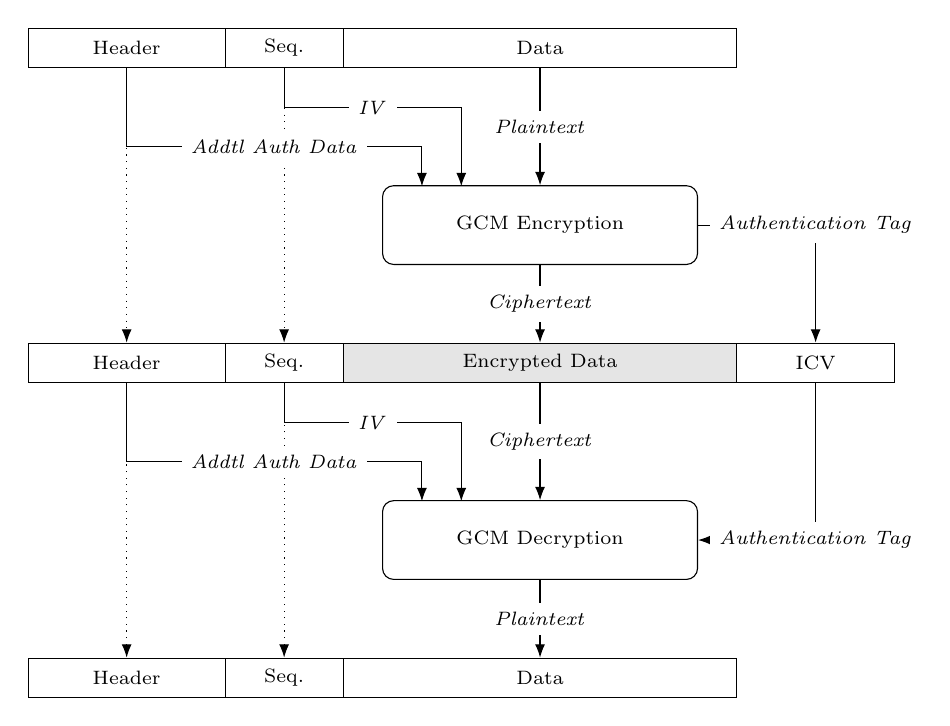
\begin{tikzpicture}[>=Latex, x=1cm, y=1cm, font=\scriptsize]
\node[rectangle,draw,minimum width=2.5cm,minimum height=.5cm] (hdr) at (1.75,4.25) {Header};
\node[rectangle,draw,minimum width=1.5cm, minimum height=.5cm] (seq) at (3.75,4.25) {Seq.};
\node[rectangle,draw,minimum width=5cm, minimum height=.5cm] (data) at (7,4.25) {Data};

% GCM Encryption box
\node[rectangle,draw,rounded corners, minimum width=4cm, minimum height=1cm] (gcm) at (7,2) {GCM Encryption};
% Bottom bar: Header | Seq. | Encrypted Data | ICV
\node[rectangle,draw,minimum width=2.5cm,minimum height=.5cm] (hdr2) at (1.75,.25) {Header};
\node[rectangle,draw,minimum width=1.5cm, minimum height=.5cm] (seq2) at (3.75,.25) {Seq.};
\node[rectangle,draw,fill=gray!20,minimum width=5cm, minimum height=.5cm] (enc) at (7,.25) {Encrypted Data};
\node[rectangle,draw,minimum width=2cm, minimum height=.5cm] (icv) at (10.5,.25) {ICV};
% Plaintext arrow
\draw[->] (data.south) -- node[fill=white] {\textit{Plaintext}} (gcm.north);
% Pass‐through dashed lines for Header & Seq
\draw[->, dotted] (hdr.south) -- (hdr2.north);
\draw[->, dotted] (seq.south) -- (seq2.north);
% IV arrow
\draw[->] (seq.south) -- ++(0,-.5) -- ++(2.25,0) node[midway, fill=white] {\textit{IV}} -- ++(0,-1);
% Additional‐Auth‐Data (dashed)
\draw[->] (hdr.south) -- ++(0,-1) -- ++(3.75,0) node[midway, fill=white] {\textit{Addtl Auth Data}} --++(0,-.5);
% Ciphertext output
\draw[->] (gcm.south) -- node[fill=white] {\textit{Ciphertext}} (enc.north);
% Authentication Tag output
\draw[->] (gcm.east) -- ++(1.5,0) -| node[fill=white] {\textit{Authentication Tag}} (icv.north);
\begin{scope}[yshift=-4cm]
	% 2) Bottom bar: Header | Seq. | Data
\node[rectangle,draw,minimum width=2.5cm,minimum height=.5cm] (hdr) at (1.75,.25) {Header};
\node[rectangle,draw,minimum width=1.5cm, minimum height=.5cm] (seq) at (3.75,.25) {Seq.};
\node[rectangle,draw,minimum width=5cm, minimum height=.5cm] (data) at (7,.25) {Data};

% 3) GCM Encryption box
\node[rectangle,draw,rounded corners, minimum width=4cm, minimum height=1cm] (gcm) at (7,2) {GCM Decryption};

% 5) Plaintext arrow
\draw[<-] (data.north) -- node[fill=white] {\textit{Plaintext}} (gcm.south);

% 6) Pass‐through dashed lines for Header & Seq
\draw[<-, dotted] (hdr.north) -- (hdr2.south);
\draw[<-, dotted] (seq.north) -- (seq2.south);

% 7) IV arrow
\draw[->] (seq2.south) -- ++(0,-.5) -- ++(2.25,0) node[midway, fill=white] {\textit{IV}} -- ++(0,-1);

% 8) Additional‐Auth‐Data (dashed)
\draw[->] (hdr2.south) -- ++(0,-1) -- ++(3.75,0) node[midway, fill=white] {\textit{Addtl Auth Data}} --++(0,-.5);

% 9) Ciphertext output
\draw[<-] (gcm.north) -- node[fill=white] {\textit{Ciphertext}} (enc.south);

% 10) Authentication Tag output
\draw[<-] (gcm.east) --  ++(1.5,0) -| node[fill=white] {\textit{Authentication Tag}} (icv.south);
\end{scope}
\end{tikzpicture}
\end{document}
